\documentclass[11pt]{article}
\usepackage[margin=1in]{geometry}
\usepackage{mathpazo}
\usepackage{amsmath,amssymb}
\usepackage{microtype}
\usepackage{booktabs}
\usepackage{graphicx}
\usepackage[dvipsnames]{xcolor}
\usepackage{tikz}
\usetikzlibrary{positioning,arrows.meta,calc,fit,backgrounds}
\usepackage[most]{tcolorbox}
\usepackage{enumitem}
\usepackage{listings}
\usepackage[font=small,labelfont=bf]{caption}
\usepackage{hyperref}
\hypersetup{colorlinks=true,linkcolor=MidnightBlue,citecolor=MidnightBlue,urlcolor=MidnightBlue}
\usepackage{cleveref}
\urlstyle{tt}
\def\UrlBreaks{\do\_\do/\do.}
\newcommand{\file}[1]{\nolinkurl{#1}}
\newcommand{\code}[1]{\texttt{#1}}
\newcommand{\mhh}{m_{hh}}
\newcommand{\bw}{\boldsymbol{\omega}}
\newcommand{\bp}{\boldsymbol{p}}
\newcommand{\bx}{\boldsymbol{x}}
\newcommand{\data}{\mathcal{D}}

\definecolor{trainable}{HTML}{1B6CA8}
\definecolor{physics}{HTML}{2E933C}
\definecolor{datac}{HTML}{7B4EA3}
\definecolor{warn}{HTML}{C0392B}

\newtcolorbox{keyidea}[1][]{enhanced,breakable,colback=physics!6,colframe=physics!70!black,
  fonttitle=\bfseries,title={#1},boxrule=0.6pt,arc=2pt,left=6pt,right=6pt}
\newtcolorbox{aside}[1][]{enhanced,breakable,colback=trainable!5,colframe=trainable!70!black,
  fonttitle=\bfseries,title={#1},boxrule=0.6pt,arc=2pt,left=6pt,right=6pt}
\newtcolorbox{assume}[1][]{enhanced,breakable,colback=datac!5,colframe=datac!70!black,
  fonttitle=\bfseries,title={#1},boxrule=0.6pt,arc=2pt,left=6pt,right=6pt}
\newtcolorbox{watch}[1][]{enhanced,breakable,colback=warn!5,colframe=warn!70!black,
  fonttitle=\bfseries,title={#1},boxrule=0.6pt,arc=2pt,left=6pt,right=6pt}
\setlist{itemsep=2pt,topsep=3pt}
\setlength{\emergencystretch}{3em}

\lstset{language=Python, basicstyle=\ttfamily\small, columns=fullflexible,
  keepspaces=true, commentstyle=\color{physics!70!black}\itshape,
  keywordstyle=\color{trainable!90!black}\bfseries, stringstyle=\color{datac},
  showstringspaces=false, frame=single, rulecolor=\color{gray!40},
  backgroundcolor=\color{gray!3}, xleftmargin=4pt, xrightmargin=4pt,
  aboveskip=6pt, belowskip=6pt}

\title{\textbf{A robust, noise-weighted loss for \texttt{HEFTNet}}\\[4pt]
\large Plan for the Huber-pull fine-tune: one model first, then the ensemble\\[4pt]
\normalsize For approval before any code is written}
\date{October 31, 2026}

\begin{document}
\maketitle

\begin{abstract}
\noindent
The BNN runs showed that weighting each bin by its POWHEG noise, starting from the L1
solution and using full-data gradients, cuts the mean $\chi^2$ per bin near threshold from
8.4 to 1.9; the bootstrap ensemble showed that an ensemble of L1 models is well calibrated
but keeps the threshold bias (\file{docs/bnn/bnn_run3.pdf}). This plan describes how to
obtain both in one procedure, suitable as the headline result of a paper: every network is
trained in two stages, the usual L1 training followed by a short fine-tune with the
\emph{Huber loss applied to the pulls}, the residuals in units of the POWHEG noise. The
first step, described in detail here, tests the fine-tune on a single model for several
values of the Huber threshold $\delta$, in a new notebook \file{code/heft_finetune.ipynb}
with a small new module \file{dihiggs/finetune.py}. If it works, the ensemble notebook gains
a fine-tune stage (\cref{sec:after}). Nothing is written until you approve; the decisions
are collected in \cref{sec:decisions}.
\end{abstract}

\begin{keyidea}[The proposal in brief]
\begin{enumerate}
  \item \textbf{The loss:} $\ell_\delta(r_k)$, the Huber function of the pull
    $r_k = (f_k - t_k)/\sigma_k$; quadratic ($\chi^2$) for $|r_k| \le \delta$, linear
    beyond. $\sigma_k$ is the POWHEG noise of the bin.
  \item \textbf{Two stages:} start from a trained L1 model; fine-tune with full-batch
    gradients, Adam at a small learning rate, saving the parameters with the best
    validation loss (the same loss, on the validation rows).
  \item \textbf{No second target column:} each row's noise variance is a separate tensor,
    aligned with the rows; batches are formed by row \emph{indices}, which pick out the
    inputs, the targets and the variances together.
  \item \textbf{The test:} $\delta = 1, 2, 3$ and $\infty$ (plain $\chi^2$), from
    \file{runs/L1Loss}, compared on the 1,000 holdout spectra with the L1 model and the
    full-data BNN. A few minutes on the 5090.
  \item \textbf{Success:} threshold $\chi^2$ per bin close to the BNN's 1.9, no loss of
    accuracy above 555 GeV, fewer negative predictions.
\end{enumerate}
\end{keyidea}

\tableofcontents

% ===========================================================================
\section{The loss}
\label{sec:loss}

\subsection{Huber on the pulls}

For a training row $k$ with POWHEG value $t_k$, prediction $f_k$ and noise variance
$\sigma_k^2$, define the pull $r_k = (f_k - t_k)/\sigma_k$ and minimise the average of
\begin{equation}
  \ell_\delta(r) = \begin{cases} \tfrac12 r^2, & |r| \le \delta,\\[2pt]
  \delta\,\bigl(|r| - \tfrac12\delta\bigr), & |r| > \delta. \end{cases}
  \label{eq:huber}
\end{equation}
The two pieces join smoothly at $|r| = \delta$: same value, same slope. $\delta$ is
measured in units of the noise: with $\delta = 2$, a bin within two standard deviations of
POWHEG contributes its $\chi^2$, and a bin further away contributes only linearly.

\begin{figure}[h]
\centering
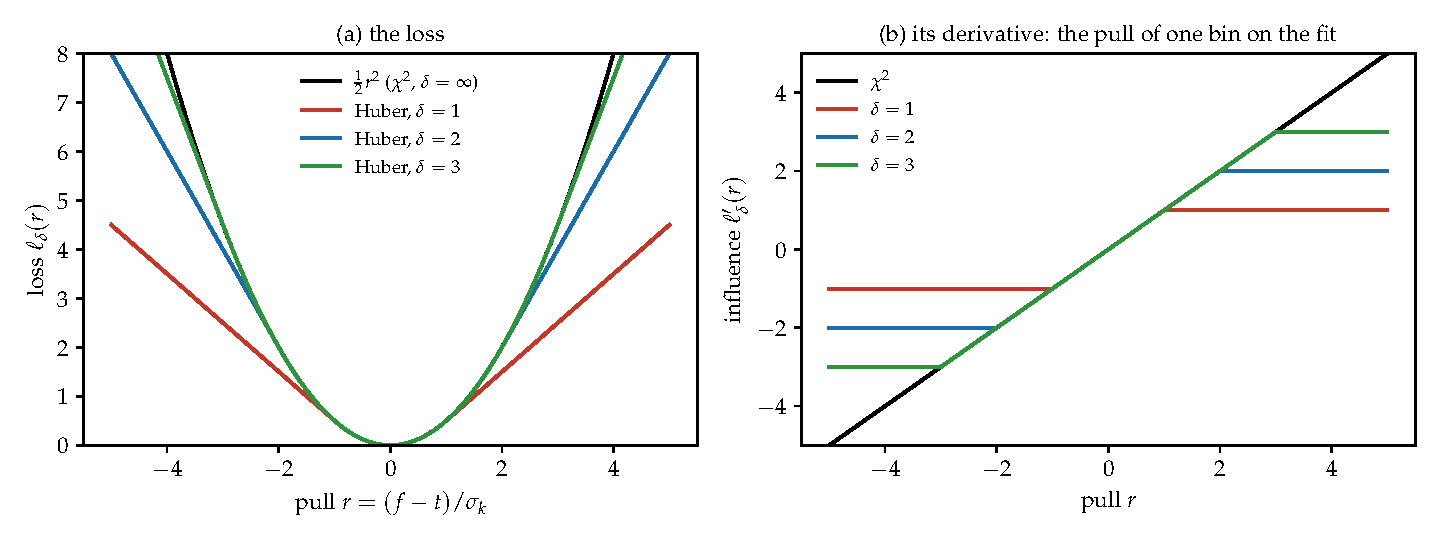
\includegraphics[width=\textwidth]{fig_huber.pdf}
\caption{(a) The Huber loss for $\delta = 1, 2, 3$, and $\tfrac12 r^2$ ($\chi^2$,
$\delta = \infty$). (b) Its derivative, the ``influence'' of one bin: how hard that bin
pulls the fit towards itself. For $\chi^2$ the influence grows without limit with the
pull; for Huber it is capped at $\pm\delta$.}
\label{fig:huber}
\end{figure}

\begin{aside}[Why on the pulls and not on the residuals in pb]
Huber applied to $f_k - t_k$ in pb interpolates between MSE and L1, and keeps their
weakness: an error of $10^{-4}$~pb counts the same in every bin, so the large cross sections
dominate and the region just above threshold, where the cross section is $10^{-2}$ of its
peak, is neglected. What the BNN showed is that the remedy is to measure each error in
units of that bin's noise, as $\chi^2$ does. Huber on the pulls keeps exactly that for the
well-modelled bins, which are the vast majority.
\end{aside}

\subsection{What the linear tails buy}

\begin{itemize}
  \item \textbf{Robustness.} A bin with a large pull, from a mismodelled region, one of the
    ten incomplete POWHEG runs, or an underestimated noise, pulls the fit with a force of
    at most $\delta$, not $|r_k|$ (\cref{fig:huber}b). The pulls of the BNN and the
    ensemble have heavier tails than a Gaussian (\file{bnn_run3.pdf}, Fig.~3), so this is
    not hypothetical.
  \item \textbf{Gentler start.} Early in the fine-tune many pulls near threshold are large
    (the L1 model's threshold $\chi^2$ is 8.4 per bin). With Huber, those bins enter
    linearly at first and quadratically once they are fitted. The gradient of a bin is
    capped at $\delta/\sigma_k$; $1/\sigma_k$ still spans several decades, so this eases
    the conditioning problem of the plain CHI2 loss without removing it, which is why the
    fine-tune also starts from the L1 solution (\cref{sec:stages}).
  \item \textbf{One story with the BNN.} For $|r_k| \le \delta$ the loss is the Poisson
    likelihood of the BNN (a Gaussian with the known variance). The BNN then cross-checks
    the same fit, not a different one.
\end{itemize}

\noindent Including $\delta = \infty$ (plain $\chi^2$) in the test shows whether the tails
matter in practice.

\subsection{The noise of each bin}
\label{sec:noise}

As in \file{heft_train.ipynb} (before the CHI2 loss was removed) and the BNN notebook: each
spectrum behaves as a histogram of about $N_\text{eff} \approx 38{,}000$ equal-weight
events, estimated from the bin-to-bin jitter of the \emph{training} spectra, and each bin
is given the variance of one extra event so that no bin claims to be known better than
that:
\begin{equation}
  \sigma_k^2 = \Bigl(t_k + \frac{\sigma_\text{tot}}{N_\text{eff}}\Bigr)
               \frac{\sigma_\text{tot}}{N_\text{eff}},
  \label{eq:noise}
\end{equation}
where $\sigma_\text{tot}$ is the total cross section of the spectrum to which the row
belongs.

\begin{watch}[Variance from the data or from the model?]
Equation (\ref{eq:noise}) uses the observed $t_k$. A bin that fluctuates down then gets a
smaller $\sigma_k$, a larger weight, and pulls the fit slightly low, by a relative amount
of order $1/n_k$, the inverse of the number of events in the bin (Neyman's $\chi^2$). The
alternative is to use the model's own prediction, held fixed during each step
(\code{f.detach()}), in place of $t_k$ (Pearson's $\chi^2$), which removes that bias but
makes the weights move during the fit. The bias matters only for bins with very few events.
I propose the observed $t_k$ for the test, as in the BNN's Poisson likelihood, so that the
two are comparable, with a switch \code{VARIANCE\_FROM = 'data' | 'model'} to try the other
(\cref{sec:decisions}).
\end{watch}

% ===========================================================================
\section{Two stages}
\label{sec:stages}

\paragraph{Why not train with this loss from the start.} The CHI2 loss failed when trained
from random weights with mini-batches of 2,048 (\file{dihiggs_report.pdf}): median holdout
$\chi^2/N$ 382 after 20,000 iterations against 3.8 for L1. In the BNN runs the same
weighting worked well, starting from the L1 solution and with every gradient computed on
all the training rows. The fine-tune reproduces those two conditions.

\paragraph{Stage 1} is the L1 training of \file{heft_train.ipynb}, unchanged. For the test,
stage 1 is the existing model \file{runs/L1Loss}, the same start as every BNN run, so the
comparison with the full-data BNN is direct.

\paragraph{Stage 2, the fine-tune.}
\begin{itemize}
  \item \textbf{Full-batch gradients:} each step uses all 274,152 training rows (in chunks
    of, say, 65,536, whose gradients add up exactly, as in \code{hmc.Posterior}). About 4
    ms per step on the 5090, 0.3 s on a laptop CPU.
  \item \textbf{Adam,} learning rate $10^{-4}$ halved every 1,250 steps, 5,000 steps in all
    (switches \code{FT\_LR}, \code{FT\_STEPS}). Adam rescales each parameter's step by its
    own gradient history, which helps with the spread of scales.
  \item \textbf{Validation:} every 50 steps the same loss is computed on the validation rows
    of \file{heft_train.ipynb}, and the parameters with the lowest value are kept; the loss
    history is written to \file{dihiggs_losses.csv} as usual.
  \item \textbf{Divergence guard:} if the training loss becomes non-finite, the fine-tune
    stops and keeps the best parameters so far.
\end{itemize}

% ===========================================================================
\section{Carrying the noise without a second target}
\label{sec:carry}

The loss needs $\sigma_k$ for every row of a batch, and the noise variance must not be a
second target column. The fine-tune therefore does not use \code{drwho}'s
\code{DataLoader}, which hands out (inputs, targets) only. Instead:
\begin{enumerate}
  \item three tensors, on the GPU, aligned row by row: inputs \code{X} [$N$, 6], targets
    \code{T} [$N$], noise variances \code{V} [$N$];
  \item a batch is a set of row \emph{indices} \code{idx}; the batch is then
    \code{X[idx]}, \code{T[idx]}, \code{V[idx]};
  \item with full-batch gradients, the ``batches'' are simply consecutive chunks of the
    rows, and \code{idx} is a slice.
\end{enumerate}
The target remains the cross section alone; the variance is a known property of each row,
handed to the loss beside it, exactly as \code{hmc.PoissonLikelihood} receives it.
\code{V} is computed once, from Eq.~(\ref{eq:noise}), from the training file itself; for
\code{VARIANCE\_FROM = 'model'} only the $\sigma_\text{tot}/N_\text{eff}$ part is stored and
the $t_k$ in Eq.~(\ref{eq:noise}) is replaced by the detached prediction.

% ===========================================================================
\section{The code}
\label{sec:code}

\subsection{\texttt{dihiggs/finetune.py}}

A small module, commented in the style of \file{hmc.py}, importing nothing from the rest of
\code{dihiggs} except what is passed in:

\begin{center}
\small
\begin{tabular}{p{0.32\textwidth}p{0.62\textwidth}}
\toprule
function / class & what it does\\
\midrule
\code{estimate\_n\_eff(df)} & $N_\text{eff}$ from the bin-to-bin jitter of the spectra in a
  training data frame (the code now repeated in three notebooks)\\
\code{noise\_variance(df, n\_eff)} & Eq.~(\ref{eq:noise}) for every row; also returns
  $\sigma_\text{tot}/N_\text{eff}$\\
\code{HuberPull(delta)} & the loss (\ref{eq:huber}) of predictions $f$, targets $t$,
  variances $v$, averaged; \code{delta=None} gives $\tfrac12 r^2$\\
\code{finetune(model, X, T, V, Xv, Tv, Vv, ...)} & stage 2: full-batch Adam with the
  learning-rate steps, validation every 50 steps, best-parameter saving, loss file; returns
  the loss history\\
\bottomrule
\end{tabular}
\end{center}

\subsection{\texttt{code/heft\_finetune.ipynb}}

In the style of \file{heft_train.ipynb} (header, Colab cell, imports, device, data with its
SHA-256), then:
\begin{enumerate}
  \item \textbf{Introduction:} the loss, the pulls, the two stages (condensed from
    \cref{sec:loss,sec:stages}).
  \item \textbf{Switches:} \code{START = 'runs/L1Loss/dihiggs\_params.pth'};
    \code{DELTAS = [1, 2, 3, None]} (\code{None} = $\chi^2$);
    \code{VARIANCE\_FROM = 'data'}; \code{FT\_STEPS = 5000}; \code{FT\_LR = 1e-4};
    \code{SEED = 42}.
  \item \textbf{The split} of \file{heft_train.ipynb}; $N_\text{eff}$ and the variances.
  \item \textbf{The fine-tunes:} one per value of $\delta$, each from the same starting
    model, saved in \file{runs/FT_huber_d1/}, \file{FT_huber_d2/}, \file{FT_huber_d3/},
    \file{FT_chi2/}: an ordinary run folder (configuration with $\delta$, $N_\text{eff}$,
    the schedule and the starting file; \file{dihiggs_params.pth}; the loss file), so that
    \file{heft_test.ipynb} and \file{heft_export.ipynb} work with any of them.
  \item \textbf{Results on the holdout spectra} (\cref{sec:test}).
\end{enumerate}

% ===========================================================================
\section{The test}
\label{sec:test}

On the 1,000 holdout spectra, for the starting L1 model, each fine-tuned model and, if its
folder is present, the full-data BNN mean:

\begin{center}
\small
\begin{tabular}{p{0.38\textwidth}p{0.54\textwidth}}
\toprule
quantity & why\\
\midrule
mean $\chi^2$ per bin, 255--555 GeV & the target of the exercise (L1: 8.4; BNN: 1.9)\\
mean $\chi^2$ per bin, above 555 GeV & must not get worse (L1: 1.20; BNN: 1.12)\\
median $\chi^2/N$; fractions above 2 and 5 & overall accuracy, and the bad spectra\\
mean $|$residual$|$ in pb & what L1 optimises; a small loss here is expected\\
negative predictions & physical sanity\\
$\chi^2$ per bin against $\mhh$ (figure) & where the gains and losses are\\
the loss curves (figure) & that the fine-tune converged, without overfitting\\
\bottomrule
\end{tabular}
\end{center}

\paragraph{What counts as success.} A value of $\delta$ for which the threshold $\chi^2$
per bin is close to the BNN's 1.9, the $\chi^2$ above 555 GeV is no worse than the L1
model's, and negative predictions are fewer. If $\delta = \infty$ does as well as finite
$\delta$, the robustness argument still favours a finite value; if it does clearly worse,
the tails matter. If no value succeeds, the next things to try are a smaller learning rate,
more steps, and \code{VARIANCE\_FROM = 'model'}.

\paragraph{Cost.} Four fine-tunes of 5,000 full-batch steps: about 1.5 minutes on the 5090
(about two hours on a laptop CPU, so the 5090 is the place for it).

% ===========================================================================
\section{After the test}
\label{sec:after}

\begin{enumerate}
  \item \textbf{The ensemble with the chosen $\delta$.} \file{heft_train_ensemble.ipynb}
    gains a switch \code{FINETUNE\_DELTA} (default \code{None}: no fine-tune, as now). With
    a value, each member, after its L1 training, is fine-tuned on \emph{its own} bootstrap
    rows, and saved as before; the stage-1 parameters are kept as
    \file{dihiggs_params_L1.pth}. The fine-tune adds well under a minute per member on the
    5090. Then the bootstrap and \code{'seeds'} ensembles are trained this way.
  \item \textbf{The test of the ensemble} is that of \file{bnn_run3.pdf}: accuracy and the
    pull. Success: as accurate as the BNN, as well calibrated as the L1 ensemble.
  \item \textbf{The BNN cross-check:} the full-data Poisson BNN with the fixed warm-up,
    started from the fine-tuned model rather than the L1 model (shorter descent).
\end{enumerate}

% ===========================================================================
\section{Not in this plan}
\begin{itemize}
  \item No change to \file{heft_train.ipynb}, \file{heft_test.ipynb}, \file{hmc.py} or the
    data. The three notebooks that estimate $N_\text{eff}$ keep their own code for now;
    they can later call \code{finetune.estimate\_n\_eff}.
  \item The changes to \file{heft_train_ensemble.ipynb} of \cref{sec:after}, which wait
    for the result of the test.
  \item Exact per-spectrum event weights $w_j$ (recoverable from the quantization of the
    spectra) instead of the $N_\text{eff}$ estimate: a later refinement.
  \item Nothing is committed to git.
\end{itemize}

% ===========================================================================
\section{Decisions for you}
\label{sec:decisions}

\begin{keyidea}[Decisions before I proceed]
\begin{enumerate}
  \item \textbf{Huber on the pulls} (not on the residuals in pb), with
    $\delta \in \{1, 2, 3, \infty\}$ in the test. Agreed?
  \item \textbf{Two stages,} starting the test from \file{runs/L1Loss}. Agreed?
  \item \textbf{Full-batch Adam,} $10^{-4}$ halved every 1,250 steps, 5,000 steps, best
    validation loss kept. Agreed, or would you prefer large mini-batches?
  \item \textbf{The noise as a separate tensor} indexed with the rows (not a target column).
    Agreed?
  \item \textbf{Variance from the data} for the test, with the \code{'model'} option
    available. Agreed?
  \item \textbf{A new module and notebook,} \file{dihiggs/finetune.py} and
    \file{code/heft_finetune.ipynb}; folders \file{runs/FT_huber_d<delta>/},
    \file{runs/FT_chi2/}. Acceptable?
  \item \textbf{Location of this document:} \file{docs/huber/huber_plan.pdf}?
\end{enumerate}
\end{keyidea}

\end{document}
